\documentclass[conference]{IEEEtran} 
\IEEEoverridecommandlockouts
\usepackage{cite}
\usepackage{amsmath,amssymb,amsfonts}
\usepackage{algorithmic}
\usepackage{flafter}
\usepackage{graphicx}
\usepackage{textcomp}
\usepackage{xcolor}
\graphicspath{ {imagenes/} }

\begin{document}

\title{Actividad G.5 \\ Terminal }

\author{\IEEEauthorblockN{Ricardo David López Arellano}
\IEEEauthorblockA{\textit{Departamento de Ingeniería en Computación} \\
\textit{CUCEI}\\
Universidad de Guadalajara\\
ricardo.lopez1361@alumnos.udg.mx} }
\onecolumn

\maketitle

\begin{abstract}
Se denomina terminal o consola (hardware) a un dispositivo electrónico o electromecánico que se utiliza para interactuar con un computador.
\end{abstract}

\begin{IEEEkeywords}
\begin{center}
Cursor, OS:gotoxy, OS:wherex, OS:wherey, count, cr, dup, over, getch, OS:key, 
\end{center}
\end{IEEEkeywords}

\section{Originalidad}
Me comprometo a producir trabajo académico íntegro, lo que significa un trabajo que se adhiere a los estándares intelectuales y académicos de atribución exacta de las fuentes, uso y recolección de datos apropiados, y transparencia en el reconocimiento de las contribuciones de las ideas, descubrimientos, interpretaciones y conclusiones de otros.
Acepto que la trampa en los exámenes, el plagio o la fraudulenta representación de las ideas o lenguaje de otros como propio, la falsificación de datos o cualquier otra instancia de deshonestidad académica, violan los estándares de LA MATERIA, así como los estándares del mundo en general en el campo del conocimiento y las relaciones.

\section{Introducción}
\begin{center}
Una terminal es un programa cuyo objetivo principal es leer comandos y ejecutar otros programas. Las principales ventajas de la terminal son su alta relación acción-tecla, su soporte para la automatización de tareas repetitivas, y que puede utilizarse para acceder a otras máquinas en una red.
\end{center}

\section{Objetivos de la actividad}
\begin{center}
 • Manipular la terminal mediante el uso de palabras orientadas a la misma.
\end{center}

\section{Metodología}
OS:gotoxy: es una palabra que mueve el cursor a la posición requerida (coordenadas x, y) pasadas a través de la pila de datos. \\
\\OS:wherex: regresa la coordenada 'x' de la posición del cursor en la pila de datos. \\
\\OS:wherey: regresa la coordenada 'y' de la posición actual del cursor en la pila de datos. \\
\\Count: palabra que regresa el número de símbolos que contiene el texto que se encuentra en la celda superior de la pila de direcciones. Además, es importante señalar que dicha cuenta no incluye el símbolo de terminación nulo. \\
\\cr: palabra que imprime un salto de línea en la terminal. \\
\\dup: palabra que crea una copia del texto que se encuentra en la celda superior en la pila de direcciones. \\
\\over: palabra que duplica la segunda celda en la pila de direcciones. \\
\\OS:getch: palabra que lee un byte procedente de teclado y lo guarda en la pila de datos. \\
\\OS:key: palabra que lee un símbolo (de 1 o más bytes) procedente del teclado y lo guarda en la pila de datos. \\ 

\section{Contenido}
\subsection{Estructuras:}
Entrada de usuario: \\
El usuario puede interactuar con un programa mediante diversos dispositivos, entre los cuales se encuentra el teclado, el cual está inspirado en el teclado de las máquinas de escribir, presentando diferentes disposiciones de las teclas. Por otro lado, en esta sección se abordarán las instrucciones que permiten leer las teclas presionadas por el usuario. \\
\\Texto: \\
Un texto o cadena de texto es una espacio en memoria que contiene una secuencia de símbolos (caracteres) y tiene una longitud arbitraria, terminando en un símbolo nulo equivalente a 00 hexadecimal. Además, es importante señalar que los símbolos en dicho texto pueden tener una longitud igual o mayor a un byte. Por otro lado, para introducir un texto se deben poner los símbolos entre comillas dobles, por ejemplo, "hola mundo", donde dicha cadena de texto se guardará en la pila de apuntadores. Además, en el caso de los símbolos se escriben entre comillas simples, por ejemplo, 'a', y dichos símbolos se guardan en la pila de datos. \\
\\Cursor: \\
Se denomina terminal o consola (hadware) a un dispositivo electrónico o electromecánico que se utiliza para interactuar con un computador. Generalmente la terminal soporto códigos de escape (ESC), los cuales permiten cambiar colores, mover el cursor, entre otros. Además, dichos códigos se pueden utilizar mediante un texto enviado a la terminal que contiene "ESC[7m". donde después del corchete cuadrado se debe especificar el código a utilizar. Por otro lado, en esta sección se abordarán las instrucciones que permiten mover el cursor en la terminal.

\section{Resultados}
\begin{enumerate}
\item  EJERCICIO 1:\\
	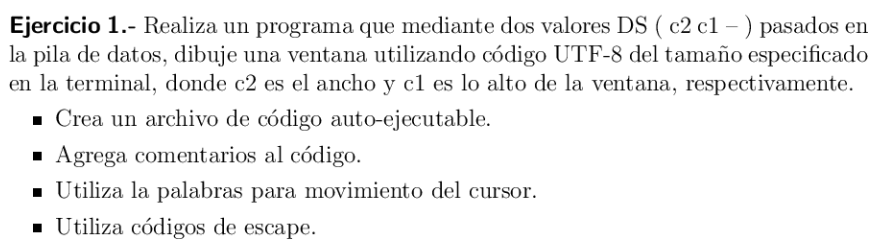
\includegraphics{e1} \\
	\begin{center}
	\textbf{Respuesta: } 20       	//ALTO \\ 80       	//ANCHO \\ 2 - //restamos 2 caracteres a la pila \\ (las orillas superiores) \\ swap \\ 2 - //restamos 2 caracteres a la pila (las orillas inferiores) \\ swap \\ "+" S. //Ingresamos la orilla superior izquierda \\ dup \\ 2 / \\ 8 - \\ dup \\ while dup 0 > \\ //ciclo para hacer linea superior \\  "-" S. \\  1 - \\ drop \\ dup \\ while dup 0 > //ciclo para hacer \\ linea inferior \\  "-" S. \\  1 - \\ drop \\ swap \\ "+" S. //Ingresamos la orilla superior derecha \\ cr \\ swap \\ drop \\ swap \\ dup \\ swap \\ rot \\ swap \\ while dup 0 > //ciclo para hacer lineas de los costados \\ "¦" S. //primer linea izquierda del primer renglón \\   swap \\   dup \\ while dup 0 > \\   " " S. //Imprimir espacios \\   1 - \\   drop \\   swap \\   1 - \\   "¦" S. //Linea final del primer renglón \\   cr \\ drop \\ "+" S. //Ingresamos la orilla inferior izquierda \\ dup \\ while dup 0 > \\ //ciclo de la linea final \\  "-" S. \\  1 - \\ swap \\ "+" S. //Ingresamos la orilla inferior derecha \\ swap \\ drop \\ cr \\ drop 
	\end{center}
\newpage
\item  EJERCICIO 2:\\
	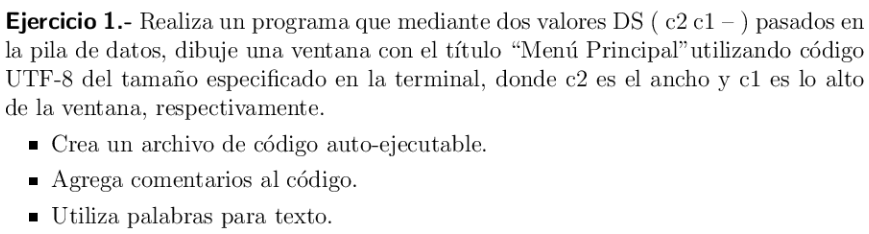
\includegraphics{e2} \\
	\begin{center}
	\textbf{Respuesta: }  20       	//ALTO \\ 80       	//ANCHO \\ 2 - //restamos 2 caracteres a la pila (las orillas superiores) \\ swap \\ 2 - //restamos 2 caracteres a la pila (las orillas inferiores) \\ swap \\ "+" S. //Ingresamos la \\ orilla superior izquierda \\ dup \\ 2 / \\ 8 - \\ dup \\ while dup 0 > //ciclo para hacer linea superior \\  "-" S. \\  1 - \\ drop \\ "¦" S. //simbolo antes de finalizar la palabra 'principal' \\ " MenuPrincipal " S. //palabras puestas de 'titulo' \\ "+" S. //simbolo antes de comenzar la palabra 'menu' \\ dup \\ while dup 0 > //ciclo para hacer linea inferior \\  "-" S. \\  1 - \\ drop \\ swap \\ "+" S. //Ingresamos la orilla superior derecha \\ cr \\ swap \\ drop \\ swap \\ dup \\ swap \\ rot \\ swap \\ while dup 0 > //ciclo para hacer lineas de los costados \\ "¦" S. //primer linea izquierda del primer renglón \\   swap \\   dup \\   while dup 0 > \\ " " S. //Imprimir espacios \\   1 - \\   drop \\   swap \\   1 - \\   "¦" S. //Linea final del primer renglón \\   cr \\ drop \\ "+" S. //Ingresamos la orilla inferior izquierda \\ dup \\ while dup 0 > //ciclo de la linea final \\  "-" S.  \\  1 - \\ swap \\ "+" S. //Ingresamos la  orilla inferior derecha \\ swap \\ drop \\ cr \\ drop
	\end{center}
	
\item  EJERCICIO 3:\\
	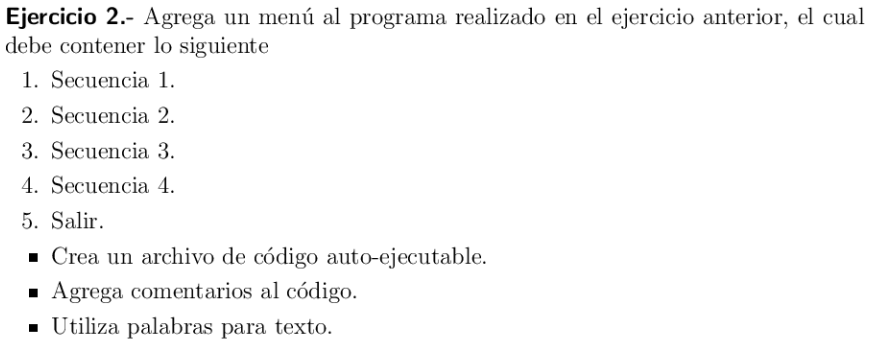
\includegraphics{e3} \\
	\begin{center}
	\textbf{Respuesta: }  //----------------- INICIA RECUADRO ------------- \\ 10       	//ALTO \\ 80       	//ANCHO \\ 2 - //restamos 2 caracteres a la pila (las orillas superiores) \\ swap \\ 2 - //restamos 2 caracteres a la pila (las \\ orillas inferiores) \\ swap \\ "+" S. //Ingresamos la orilla superior izquierda \\ dup \\ 2 / \\ 8 - \\ dup \\ while dup 0 > //ciclo para hacer linea superior \\  "-" S. \\  1 - \\ drop \\ "¦" S. //simbolo antes de finalizar la palabra  'principal' \\ " MenuPrincipal " S. //palabras puestas de 'titulo' \\ "+" S. //simbolo antes de comenzar la palabra 'menu' \\ dup \\ while dup 0 > //ciclo para hacer linea inferior \\  "-" S. \\  1 - \\ drop \\ swap \\ "+" S. \\ //Ingresamos la orilla superior derecha \\ cr \\ swap \\ drop \\ swap \\ dup \\ swap \\ rot \\ swap \\ while dup 0 > //ciclo para hacer lineas de los costados \\   "¦" S. //primer linea izquierda del primer renglón \\   swap \\ dup \\   while dup 0 > \\   " " S. //Imprimir espacios \\   1 - \\   drop \\   swap \\   1 - \\   "¦" S. //Linea final del primer renglón \\   cr \\ drop \\ "+" S. //Ingresamos la orilla inferior izquierda \\ dup \\ while dup 0 > //ciclo de la linea final \\  "-" S. \\  1 - \\ swap \\ "+" S. //Ingresamos la orilla inferior derecha \\ //----------------------- ACABA RECUADRO -------- \\ //---------- INICIA MENU DE SECUENCIAS -------- \\ swap \\ drop \\ cr \\ drop \\ //las siguientes cantidades son para ubicar al puntero en dicha posición \\ 3  \\ 14 \\ OS:gotoxy //indicacion para colocar el puntero \\ "1. Secuencia 1" S. //ingresamos la palabra requerida \\ 3 \\ 15 \\ OS:gotoxy //ubicamos cursor y ponemos la palabra \\ "2. Secuencia 2" S. \\ 3 \\ 16 \\ OS:gotoxy //ubicamos cursor y ponemos la palabra \\ "3. Secuencia 3" S. \\ 3 \\ 17 \\ OS:gotoxy //ubicamos cursor y ponemos la palabra \\ "4.Secuencia 4" S. \\ 3 \\ 18 \\ OS:gotoxy //ubicamos cursor y ponemos la palabra \\ "5. Salir" S. \\ 3 - \\ dup \\ while dup 0 > \\ cr \\ 1 - \\ drop \\ drop \\ 
	\end{center}
	
\item  EJERCICIO 4:\\
	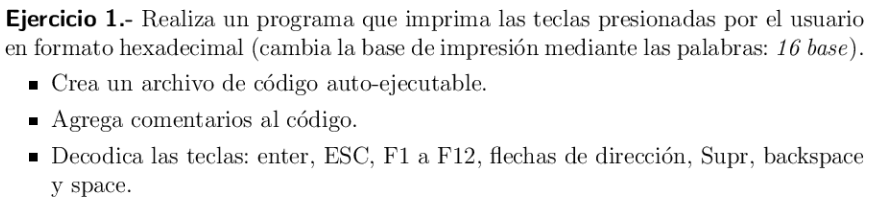
\includegraphics{e4} \\
	\begin{center}
	\textbf{Respuesta: }  16 base //al poner esto cambias los resultados a hexadecimal \\ repeat //hacemos un ciclo para que no termine hasta que presionemos la tecla de "ESC" \\ OS:key //indicacion para recibir un caracter \\ //de aqui en adelante colocaremos varios 'if' comparandolo con la tecla que se nos pidieron en su simbolo ASCII y entrando al if se imprime la tecla que hayas presionado... \\ if dup 32 = \\ dup \\ . \\ "<-ESPACIO" S. \\ cr //Con el 'cr' hacemos salto de línea para que se siga repitiendo hasta que no presionemos la tecla ESC \\ elif dup 1792833 = \\ dup \\ . \\ "<- FLECHA ARRIBA" S. \\ cr \\ elif dup 1792836 = \\ dup \\ . \\ "<- FLECHA IZQUIERDA" S. \\ cr \\ elif dup 1792834 = \\ dup \\ . \\ "<- FLECHA ABAJO" S. \\ cr \\ elif dup 1792835 = \\ dup \\ . \\ "<- FLECHA DERECHA" S. \\ cr \\ elif dup 10 = \\ dup \\ . \\ "<- ENTER" S. \\ cr \\ elif dup 127 = \\ dup \\ . \\ "<- RETROCESO" S. \\ cr \\ elif dup 458961790 = \\ dup \\ . \\ "<- SUPR" S. \\ cr \\ elif dup 1789776 = \\ dup \\ . \\ "<- F1" S. \\ cr \\ elif dup 1789777 = \\ dup \\ . \\ "<- F2" S. \\ cr \\ elif dup 1789778 = \\ dup \\ . \\ "<- F3" S. \\ cr \\ elif dup 1789779 = \\ dup \\ . \\ "<- F4" S. \\ cr \\ elif dup 458961205 = \\ dup \\ . \\ "<- F5" S. \\ cr \\ elif dup 458961207 = \\ dup \\ . \\ "<- F6" S. \\ cr \\ elif dup 458961208 = \\ dup \\ . \\ "<- F7" S. \\ cr  \\ elif dup 458961209 = \\ dup \\ . \\ "<- F8" S. \\ cr \\ elif dup 458961457 = \\ dup \\ . \\ "<- F9" S. \\ cr \\ elif dup 458961458 = \\ dup \\ . \\ "<- F10" S. \\ cr \\ elif dup 458961459 = \\ dup \\ . \\ "<- F11" S. \\ cr \\ elif dup 458961460 = \\ dup \\ . \\ "<- F12" S. \\ cr \\ until dup 27 = end \\ . \\ "<- ESC" S. \\ cr \\ 
		\end{center}
\newpage
		\item  EJERCICIO 5:\\
	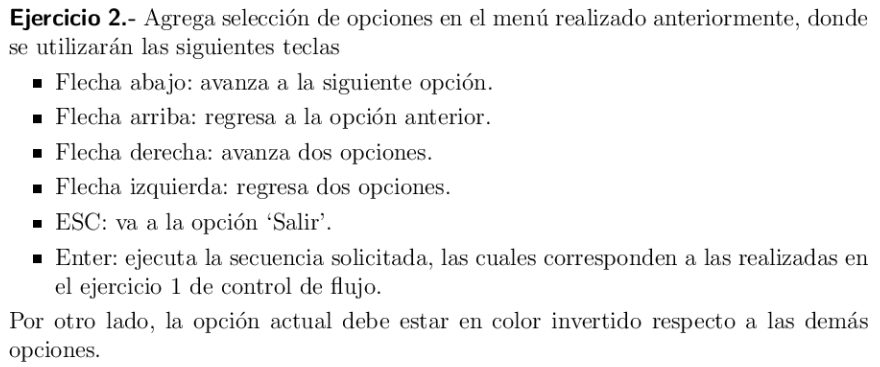
\includegraphics{e5} \\
	\begin{center}
	\textbf{Respuesta: }  ------------------ MARCO ------------------ \\ 7        	//ALTO \\ 80       	//ANCHO \\ 2 - //restamos 2 caracteres a la pila (las orillas superiores) \\ swap \\ 2 - //restamos 2 caracteres a la pila (las orillas inferiores) \\ swap \\ "+" S. //Ingresamos la orilla superior izquierda \\ dup \\ 2 / \\ 8 - \\ dup \\ while dup 0 > //ciclo para hacer linea superior \\  "-" S. \\  1 - \\ drop \\ "¦" S. //simbolo antes de finalizar la palabra 'principal' " MenuPrincipal " S. //palabras puestas de 'titulo' \\ "+" S. //simbolo antes de comenzar la palabra 'menu' \\ dup \\ while dup 0 > //ciclo para hacer linea inferior \\  "-" S. \\  1 - \\ drop \\ swap \\ "+" S. //Ingresamos la orilla superior derecha \\ cr \\ swap \\ drop \\ swap \\ dup \\ swap \\ rot \\ swap \\ while dup 0 > //ciclo para hacer lineas de los costados \\   "¦" S. //primer linea izquierda del primer renglón \\   swap \\   dup \\   while dup 0 > \\   " " S. //Imprimir espacios \\   1 - \\   drop \\   swap \\   1 - \\   "¦" S. //Linea final del primer renglón \\   cr \\ drop \\ "+" S. //Ingresamos la orilla inferior izquierda \\ dup \\ while dup 0 > //ciclo de la linea final \\  "-" S. 1 - \\ swap \\ "+" S. //Ingresamos la orilla inferior derecha \\ swap \\ drop \\ cr \\ drop \\ drop \\ //------------ IMPRIMIR MENU -------------------- \\  //iniciamos en 3 en la pila y de ahi imprimimos todas las opciones, en cada uno de los siguientes if se hará lo mismo mientras vas bajando o subiendo en el menú se seguirá impriendo el menú. (termina la programacion de menu hasta que sale el siguiente comando //------ :*) \\ 3  \\ repeat  \\ if dup 3 = \\ 3 \\ 2 \\ OS:gotoxy //ubicamos en la posicion dada anteriormente \\ "ESC[7m" S. \\ "1. Imprime del 0-9" S. \\ "ESC[0m" S. \\ 3 \\ 3 \\ OS:gotoxy \\ "2. Imprime del -9-0" S. \\ 3 \\ 4 \\ OS:gotoxy \\ "3. Imprime de la a-z" S. \\ 3 \\ 5 \\ OS:gotoxy \\ "4. Imprime de la A-Z" S. \\ 3 \\ 6 \\ OS:gotoxy \\ "5. Salir" S. \\ //pos 4 en la pila \\ elif dup 4 = \\ 3 \\ 2 \\ OS:gotoxy \\ "1. Imprime del 0-9" S. \\ 3 \\ 3 \\ OS:gotoxy \\ "ESC[7m" S. \\
	
"2. Imprime del -9-0" S. \\ "ESC[0m" S. \\ 3 \\ 4 \\ OS:gotoxy \\ "3. Imprime de la a-z" S. \\ 3 \\ 5 \\ OS:gotoxy \\ "4. Imprime de la A-Z" S. \\ 3 \\ 6 \\ OS:gotoxy \\ "5. Salir" S. \\ //pos 5 en la pila \\ elif dup 5 = \\ 3 \\ 2 \\ OS:gotoxy \\ "1. Imprime del 0-9" S. \\ 3 \\ 3 \\ OS:gotoxy \\ "2. Imprime del -9-0" S. \\ 3 \\ 4 \\ OS:gotoxy \\ "ESC[7m" S. \\ "3. Imprime de la a-z" S. \\ "ESC[0m" S. \\ 3 \\ 5 \\ OS:gotoxy \\ "4. Imprime de la A-Z" S. \\ 3 \\ 6 \\ OS:gotoxy \\ "5. Salir" S. \\ //pos 6 en la pila \\ elif dup 6 = \\ 3 \\ 2 \\ OS:gotoxy \\ "1. Imprime del 0-9" S. \\ 3 \\ 3 \\ OS:gotoxy \\ "2. Imprime del -9-0" S. \\ 3 \\ 4 \\ OS:gotoxy \\ "3. Imprime de la a-z" S. \\ 3 \\ 5 

OS:gotoxy \\ "ESC[7m" S. \\ "4. Imprime de la A-Z" S. \\ "ESC[0m" S. \\ 3 \\ 6 \\ OS:gotoxy \\ "5. Salir" S. \\ //7 en la pila (ESC) \\ elif dup 7 = \\ 3 \\ 2 \\ OS:gotoxy \\ "1. Imprime del 0-9" S. \\ 3 \\ 3 \\ OS:gotoxy \\ "2. Imprime del -9-0" S. \\ 3 \\ 4 \\ OS:gotoxy \\ "3. Imprime de la a-z" S. \\ 3 \\ 5 \\ OS:gotoxy \\ "4. Imprime de la A-Z" S. \\ 3 \\ 6 \\ OS:gotoxy \\ "ESC[7m" S. \\ "5. Salir" S. \\ "ESC[0m" S. \\ //------- :* \\ //------RESTRICCIONES --------- \\ elif dup 1 = \\ 7 + \\ elif dup 2 = \\ 6 + \\ elif dup 8 = \\ 6 - \\ elif dup 9 = \\ 7 - \\ //---------------- TECLAS -------------- \\ //en los siguientes if moveremos la posicion dependiendo la flecha que eligas... \\ OS:key \\ if dup 1792834 = \\ swap \\ 1 + \\ swap \\ drop \\ elif dup 1792833 = \\ swap \\ 1 - \\ swap \\ drop \\ elif dup 1792835 = \\ swap \\ 2 + \\ swap \\ drop \\ elif dup 1792836 = \\ swap \\ 2 - \\ swap \\ drop \\  //--------- EJERCICIOS ------------ \\ //aqui inician los ejercicios que si al dar enter haces la opcion solicitada \\ elif dup 10 = \\ drop \\ cr cr \\ //opcion 1 \\ if dup 3 = \\ 0 . \\ 0 \\ dup \\ while 9 < \\  1 + \\ dup . \\ dup \\ drop \\ //opcion 2 \\ elif dup 4 = \\ cr \\ -9 \\ while dup \\  dup S. \\ ++ \\ 0 . \\ drop \\ //opcion 3 \\ elif dup 5 = \\ cr cr \\ for 97 upto 122 \\ dup emit \\ //opcion 4 \\ elif dup 6 = \\ cr cr cr \\ 65 \\ repeat \\ dup emit \\ ++ \\ dup \\ until 91 = \\  end \\ drop \\ //opcion 5 \\ elif dup 7 = \\ jump final \\ until dup 27 = end \\ final: cr cr cr cr 
	\end{center}

\end{enumerate}

\section{Conclusiones}  
En conclusión de esta tarea puedo decir que estos ejercicios ya fueron complicados ya que su complejidad ya era mucho mas alta, se puede notar viendo el tamaño de codigo que se hizo muy extenso pero con mis conocimientos y pidiendo algo de ayuda a los compañeros pude realizarlos correctamente. Es bueno aprender un lenguaje nuevo ya que yo ni si quiera había utilizado Linux ni mucho menos Latex, así que es una buena experiencia.

\section*{Agradecimientos}
Quiero hacer agradecimiento a mi profesor por explicarme cuando tenia dudas sobre cómo hacer los ejercicios, a mis compañeros porque varias veces me brindaron ayuda cuando tenia problemas y a mis padres en apoyarme cuando los necesito.

\begin{thebibliography}{00}
\bibitem{Alvarez2022} Becerra Alvarez, E. C. (2022, 4 octubre). ForEmb. https://drive.google.com/file/d/1Jr7BqTkYkxZGCsCenfmQIbHnKNIp3zcV/view
\end{thebibliography}

\end{document}